\textbf{Выпуклые множества.}
Пусть $U$ -- вещественное векторное пространство, $Q$ -- подмножество $U$. Множество $Q$ называется \textit{выпуклым}, если для любых двух точке $x,\ y \in Q$ и любого $\lambda \in [0; 1]$ точка $\lambda x + (1 - \lambda) y$ также принадлежит множеству $Q$.

Примеры: Все пространство $U,$ множество из одного элемента, выпуклое множество, множество решений системы линейных неравенств:

\[Q := \{x\in U : \langle a_i, x\rangle \leq b_i \forall i\in I\}.\]

\begin{figure}[H]
    \centering
    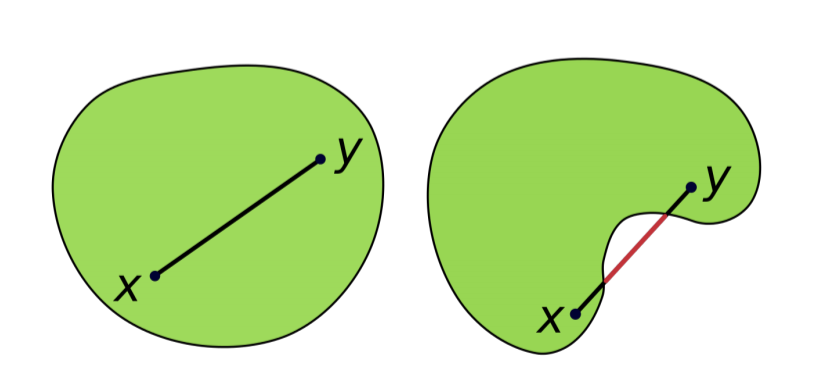
\includegraphics[width=0.5\textwidth]{images/conv_set.png}
    \caption{Слева -- выпуклое, справа -- не выпуклое.}
\end{figure}

\textbf{Свойства выпуклых функций}
\begin{enumerate}
    \item (Неравенство Йенсена) Пусть $U$ -- вещественное векторное пространство, $Q$ -- непустое выпуклое множество в $U$, и $f " Q \to \mathbb{R}$ -- выпуклая функция. Пусть также $x_1,\ldots, x_k$ -- точки в множестве $Q$ и $\lambda_1,\ldots, \lambda_k$ -- неотрицательные коэффициенты, сумммирующиеся в единицу: $\lambda_i \geq 0$ и $\sum_{i = 1}^n \lambda_i = 1.$ Тогда справедливо следующее неравенство:

    $$f\left(\sum\limits_{i= 1}^k \lambda_i x_i\right) \leq \sum_{i = 1}^k \lambda_i f(x_i),$$

    причем равенство достигается тогда и только тогда, когда функция $f$ является афинной или когда все точки совпадают: $x_1 = \ldots = x_k.$

    Другими словами, неравенство Йенсена говорит о том, для выпуклой функции значение функции от выпуклой комбинации точек не превосходит соответствующей выпуклой комбинации значений функции.

    \item(Надграфик) Пусть $U$ -- вещественное векторное пространство, $Q$ -- непустое множество в $U$. \textit{Надграфиком} функции $f : Q \to \mathbb{R}$ называется множество

    $$\mathsf{Epi}(f) := \{(x, t)\in Q \times \mathbb{R}: f(x) \leq t\}. $$
    Надграфик -- это множество из пространства $U \times \mathbb{R}.$

    \begin{figure}[H]
        \centering
        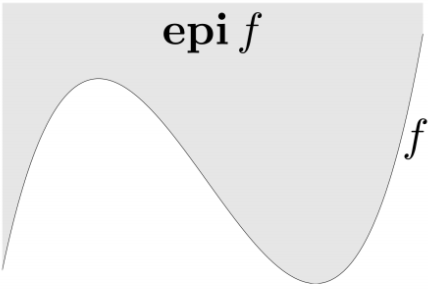
\includegraphics[width=0.5\textwidth]{images/epi.png}
        \caption{Все серое -- надграфик функции $f(x)$.}
    \end{figure}

    \textbf{Определение.} (Выпуклости через надграфик). Пусть $U$ -- вещественное векторное пространство, $Q$ -- непустое выпуклое множество в $U$. Функция $f : Q \to \mathbb{R}$ явдяется выпуклой тогда и только тогда, когда ее надграфик $\mathsf{Epi}(f)$ является выпуклым множеством в пространстве $U\times \mathbb{R}.$
    \bigskip

    \textbf{Утверждение.} (Выпуклость множества линий уровня). Пусть $U$ -- вещественное векторное пространство, $Q$ -- непустое множество в $U$, и пусть $f : Q \to \mathbb{R}$ -- выпуклая функция. Тогда для любого $\alpha \in \mathbb{R}$ соответствующее множество линий уровня

    $$\mathsf{Lev}_f(\alpha) := \{x\in Q: f(x) \leq \alpha\}$$

    является выпуклым.

    \item (Дифференциальные критерии выпуклости).\\
    \textbf{Утверждение.}(Условие выпуклости первого порядка). Пусть $Dom(f)$ является открытым множеством, и функция $f$ дифференцируема всюду на $Dom(f).$ Функция $f$ является выпуклой тогда и только тогда, когда $Dom(f)$ является выпуклым множеством и

    $$f(y) \geq f(x) + \langle\nabla f(x), y - x\rangle$$

    для всех $x,\ y\in Dom(f).$
    \bigskip

    \textbf{Утверждерние.} (Дифференциальное условие оптимальности для выпуклой функции). Пусть $f : U \to \mathbb{R}\sup \{+\infty\}$ -- выпуклая функция, $Dom(f)$ является открытым множеством, и пусть $x^* \in Dom(f).$ Тогда $x^*$ является глобальным минимумом функции $f$, если и только если $\nabla f(x^*) = 0.$ Другими словами, любая стационарная точка автоматически является глобальным минимумом функции $f.$

    \textbf{Утверждение.} (Условие выпуклости второго порядка). Пусть $Dom(f)$ является открытым множеством, и функция $f$ дважды дифференцируема на $Dom(f)$. Функция $f$ является выпуклой тогда и только тогда, когда $Dom(f)$ является выпуклым множеством и

    $$D^2f(x)[h, h] := \langle\nabla^2 f(x) h, h\rangle \geq 0$$

    для всех $x\in Dom(f)$ и всех $h\in U$. Если $U = \mathbb{R}^n,$ то это эквивалентно положительной полуопределенности гессиана:

    $$\nabla^2 f(x) \succcurlyeq 0$$

    для всех $x\in Dom(f).$

\end{enumerate}